\documentclass[tikz,border=3mm]{standalone}
\usepackage[siunitx]{circuitikz}
\usetikzlibrary{calc,positioning,arrows.meta}

\begin{document}

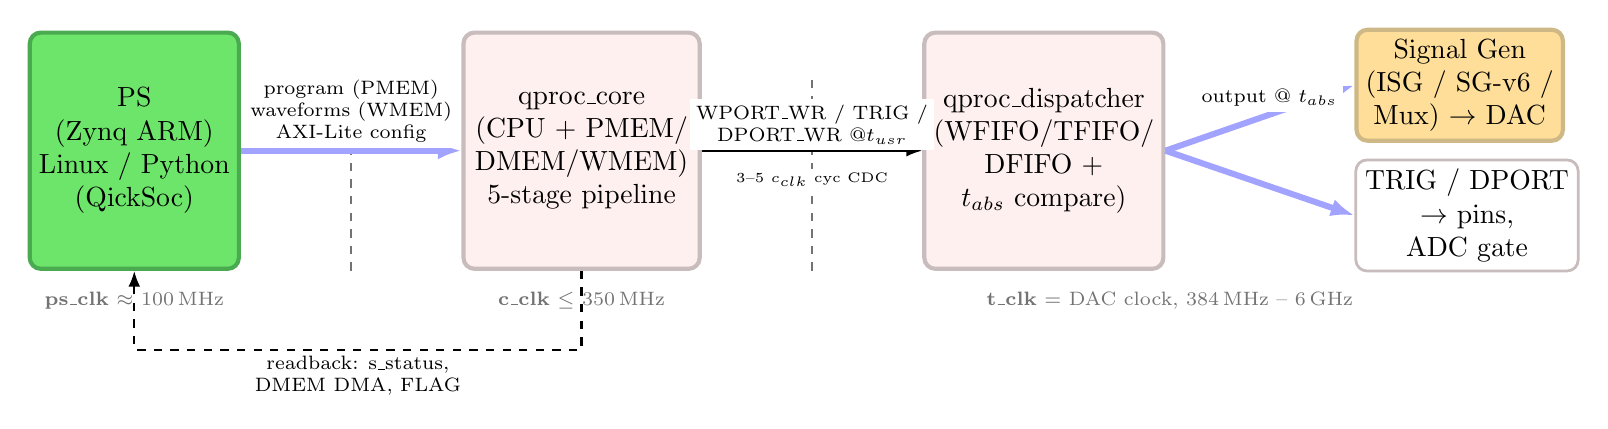
\begin{tikzpicture}
[boxRFSOCproc/.style={align=center, draw,rounded corners,minimum width=2.4cm,minimum height=3cm,draw={rgb,255:red,74; green,170; blue,80},fill={rgb,255:red,109; green,229; blue,107},line width=1.5pt},
boxtProc/.style={align=center, draw,rounded corners,minimum width=3cm,minimum height=3cm,draw={rgb,255:red,200; green,188; blue,188},fill={rgb,255:red,255; green,240; blue,240},line width=1.5pt},
boxSG/.style={align=center, draw,rounded corners,minimum width=2.6cm,minimum height=1.3cm,draw={rgb,255:red,205; green,184; blue,134},fill={rgb,255:red,254; green,222; blue,152},line width=1.5pt},
periphbox/.style={align=center, draw,rounded corners,minimum width=2.6cm,minimum height=1.3cm,draw={rgb,255:red,200; green,188; blue,188},fill=white,line width=1pt},
arrow/.style={line width=2.2pt,draw={rgb,255:red,162; green,163; blue,255},-{Latex[length=3mm]}},
single arrow/.style={line width=0.8pt,-{Latex[length=2mm]}},
node distance=0.6cm]

% Main chain: PS -> CORE -> DISPATCHER.
\node[boxRFSOCproc] (ps) {PS\\(Zynq ARM)\\Linux / Python\\(QickSoc)};

\node[boxtProc,right=2.8cm of ps] (core) {qproc\_core\\(CPU + PMEM/\\DMEM/WMEM)\\5-stage pipeline};

\node[boxtProc,right=2.8cm of core,minimum width=2.8cm] (disp) {qproc\_dispatcher\\(WFIFO/TFIFO/\\DFIFO $+$\\$t_{abs}$ compare)};

% Dispatcher outputs, stacked to the right.
\node[boxSG,above right=0.1cm and 2.4cm of disp.east] (sg) {Signal Gen\\(ISG / SG-v6 /\\Mux) $\to$ DAC};
\node[periphbox,below right=0.1cm and 2.4cm of disp.east] (trig) {TRIG / DPORT\\$\to$ pins,\\ADC gate};

% Clock-domain dividers (same convention as the PS/PL split in
% firmware-overview.tex, extended to three domains). Drawn first, so the
% (opaque, white-filled) arrow labels below sit cleanly on top of them.
\coordinate (core ps rail) at ($(core.south)+(0,-1.0)$);
\draw[black!55,thick,dashed] ($(ps.east)!0.5!(core.west)+(0,0.9)$) -- ($(ps.east)!0.5!(core.west)+(0,-1.55)$);
\draw[black!55,thick,dashed] ($(core.east)!0.5!(disp.west)+(0,0.9)$) -- ($(core.east)!0.5!(disp.west)+(0,-1.55)$);

\node[font=\scriptsize,align=center,black!55] at ($(ps)+(0,-1.9)$) {\textbf{ps\_clk} $\approx$ \SI{100}{\mega\hertz}};
\node[font=\scriptsize,align=center,black!55] at ($(core)+(0,-1.9)$) {\textbf{c\_clk} $\le$ \SI{350}{\mega\hertz}};
\node[font=\scriptsize,align=center,black!55] at ($(disp)+(1.6,-1.9)$) {\textbf{t\_clk} = DAC clock, 384\,MHz -- 6\,GHz};

% PS -> CORE: program, waveforms, AXI-Lite config (external bus, like S_AXI).
\draw[arrow] (ps.east) -- (core.west)
  node[pos=0.5,above,font=\scriptsize,align=center,fill=white,inner sep=2pt]
  {program (PMEM)\\waveforms (WMEM)\\AXI-Lite config};

% CORE -> PS: readback, routed below the boxes on a clear rail.
\draw[single arrow,dashed] (core.south) -- (core ps rail) -| (ps.south)
  node[pos=0.25,below,font=\scriptsize,align=center,fill=white,inner sep=2pt] {readback: s\_status,\\DMEM DMA, FLAG};

% CORE -> DISPATCHER: the one link that crosses the clock-domain boundary.
\draw[single arrow] (core.east) -- (disp.west)
  node[pos=0.5,above,font=\scriptsize,align=center,fill=white,inner sep=2pt]
  {WPORT\_WR / TRIG /\\DPORT\_WR @$t_{usr}$};
\node[font=\tiny,align=center,fill=white,inner sep=1.5pt,
      below=0.22cm of {$(core.east)!0.5!(disp.west)$}]
  {3--5 $c_{clk}$ cyc CDC};

% DISPATCHER -> outputs.
\draw[arrow] (disp.east) -- (sg.west)
  node[pos=0.55,above,font=\scriptsize,fill=white,inner sep=2pt] {output @ $t_{abs}$};
\draw[arrow] (disp.east) -- (trig.west);

\end{tikzpicture}

\end{document}
